\documentclass{standalone}
\usepackage{tikz}
\usetikzlibrary{patterns, positioning}


\begin{document}
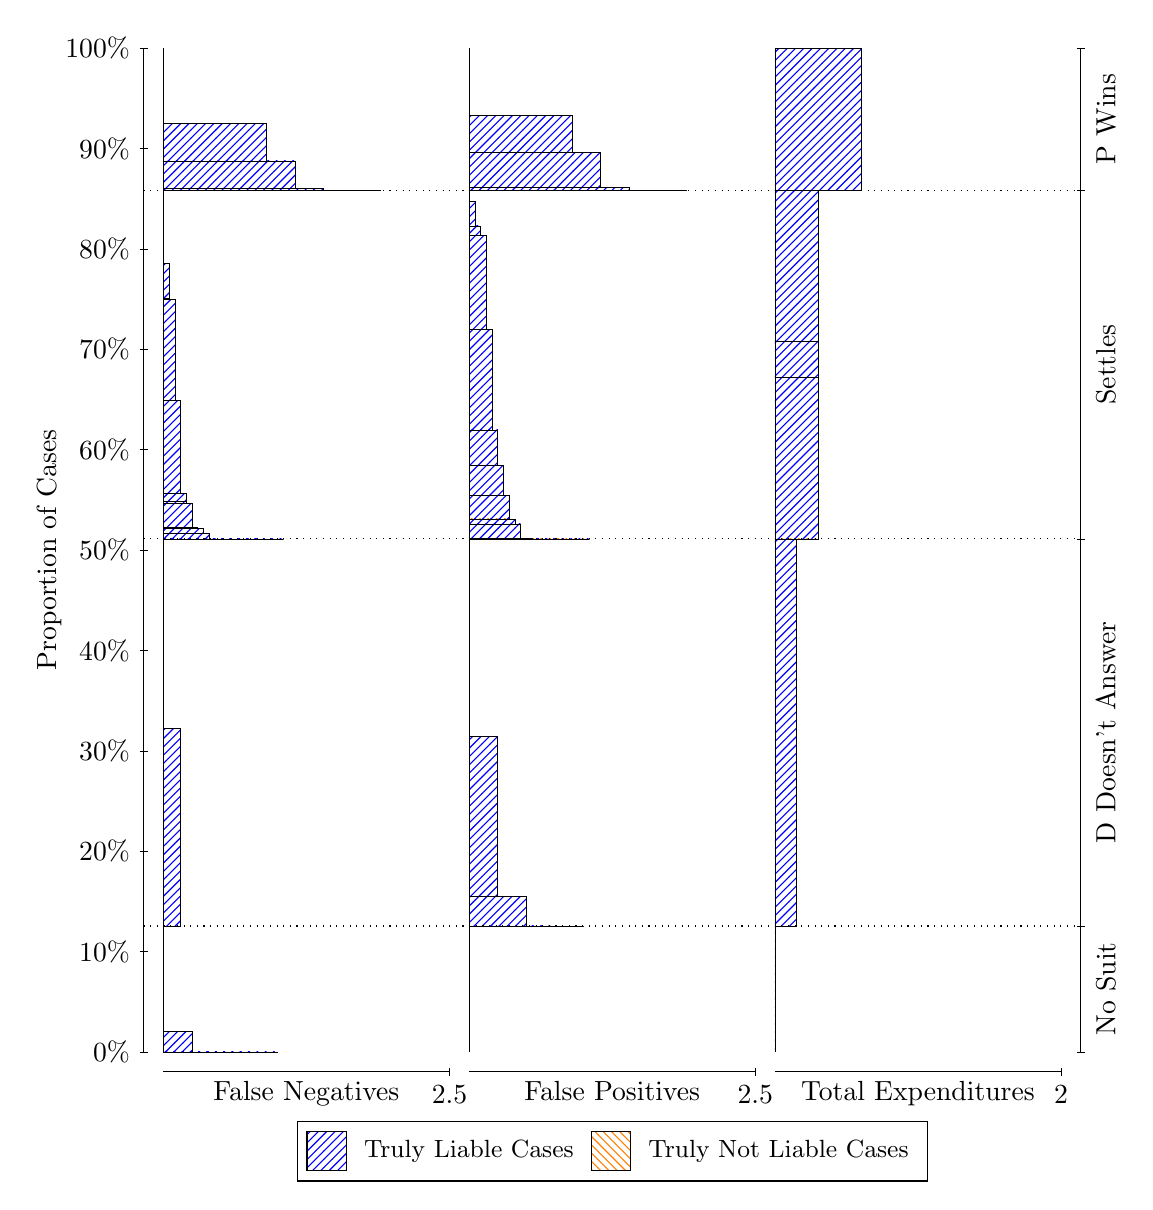
\begin{tikzpicture}
\draw[black, very thin] (1.5,1.75) -- (1.5,14.5);
\node[rotate=90, text=black, anchor=center] at (0.3, 8.125) {Proportion of Cases};
\draw[black, very thin] (1.45,1.75) -- (1.55,1.75);
\node[text=black, anchor=east] at (1.45, 1.75) {0\%};
\draw[black, very thin] (1.45,3.025) -- (1.55,3.025);
\node[text=black, anchor=east] at (1.45, 3.025) {10\%};
\draw[black, very thin] (1.45,4.3) -- (1.55,4.3);
\node[text=black, anchor=east] at (1.45, 4.3) {20\%};
\draw[black, very thin] (1.45,5.575) -- (1.55,5.575);
\node[text=black, anchor=east] at (1.45, 5.575) {30\%};
\draw[black, very thin] (1.45,6.85) -- (1.55,6.85);
\node[text=black, anchor=east] at (1.45, 6.85) {40\%};
\draw[black, very thin] (1.45,8.125) -- (1.55,8.125);
\node[text=black, anchor=east] at (1.45, 8.125) {50\%};
\draw[black, very thin] (1.45,9.4) -- (1.55,9.4);
\node[text=black, anchor=east] at (1.45, 9.4) {60\%};
\draw[black, very thin] (1.45,10.675) -- (1.55,10.675);
\node[text=black, anchor=east] at (1.45, 10.675) {70\%};
\draw[black, very thin] (1.45,11.95) -- (1.55,11.95);
\node[text=black, anchor=east] at (1.45, 11.95) {80\%};
\draw[black, very thin] (1.45,13.225) -- (1.55,13.225);
\node[text=black, anchor=east] at (1.45, 13.225) {90\%};
\draw[black, very thin] (1.45,14.5) -- (1.55,14.5);
\node[text=black, anchor=east] at (1.45, 14.5) {100\%};

\draw[black, very thin] (13.4,1.75) -- (13.4,14.5);
\draw[black, very thin] (13.35,1.75) -- (13.45,1.75);
\node[anchor=west] at (13.35, 1.75) {};
\draw[black, very thin] (13.35,3.3493) -- (13.45,3.3493);
\node[anchor=west] at (13.35, 3.3493) {};
\draw[black, very thin] (13.35,8.2665) -- (13.45,8.2665);
\node[anchor=west] at (13.35, 8.2665) {};
\draw[black, very thin] (13.35,12.695) -- (13.45,12.695);
\node[anchor=west] at (13.35, 12.695) {};
\draw[black, very thin] (13.35,14.5) -- (13.45,14.5);
\node[anchor=west] at (13.35, 14.5) {};

\draw[black, very thin, pattern color=blue, pattern=north east lines] (1.75,1.75) rectangle (3.2033,1.75);
\draw[black, very thin, pattern color=blue, pattern=north east lines] (1.75,1.75) rectangle (2.84,1.75);
\draw[black, very thin, pattern color=blue, pattern=north east lines] (1.75,1.75) rectangle (2.4767,1.7522);
\draw[black, very thin, pattern color=blue, pattern=north east lines] (1.75,1.7522) rectangle (2.1133,2.0119);
\draw[black, very thin, pattern color=orange, pattern=north west lines] (1.75,2.0119) rectangle (1.75,2.0119);
\draw[black, very thin, pattern color=blue, pattern=north east lines] (1.75,2.0119) rectangle (1.75,3.3493);
\draw[black, very thin, pattern color=blue, pattern=north east lines] (1.75,3.3493) rectangle (1.968,5.8622);
\draw[black, very thin, pattern color=orange, pattern=north west lines] (1.75,5.8622) rectangle (1.75,5.8622);
\draw[black, very thin, pattern color=blue, pattern=north east lines] (1.75,5.8622) rectangle (1.75,8.2665);
\draw[black, very thin, pattern color=blue, pattern=north east lines] (1.75,8.2665) rectangle (3.276,8.2665);
\draw[black, very thin, pattern color=blue, pattern=north east lines] (1.75,8.2665) rectangle (3.1307,8.2665);
\draw[black, very thin, pattern color=blue, pattern=north east lines] (1.75,8.2665) rectangle (2.9853,8.2665);
\draw[black, very thin, pattern color=blue, pattern=north east lines] (1.75,8.2665) rectangle (2.9127,8.2665);
\draw[black, very thin, pattern color=blue, pattern=north east lines] (1.75,8.2665) rectangle (2.84,8.2665);
\draw[black, very thin, pattern color=blue, pattern=north east lines] (1.75,8.2665) rectangle (2.7673,8.2665);
\draw[black, very thin, pattern color=blue, pattern=north east lines] (1.75,8.2665) rectangle (2.6947,8.2665);
\draw[black, very thin, pattern color=blue, pattern=north east lines] (1.75,8.2665) rectangle (2.622,8.2665);
\draw[black, very thin, pattern color=blue, pattern=north east lines] (1.75,8.2665) rectangle (2.5493,8.2665);
\draw[black, very thin, pattern color=blue, pattern=north east lines] (1.75,8.2665) rectangle (2.4767,8.267);
\draw[black, very thin, pattern color=blue, pattern=north east lines] (1.75,8.267) rectangle (2.404,8.2671);
\draw[black, very thin, pattern color=blue, pattern=north east lines] (1.75,8.2671) rectangle (2.404,8.2673);
\draw[black, very thin, pattern color=blue, pattern=north east lines] (1.75,8.2673) rectangle (2.3313,8.3313);
\draw[black, very thin, pattern color=blue, pattern=north east lines] (1.75,8.3313) rectangle (2.2587,8.3954);
\draw[black, very thin, pattern color=blue, pattern=north east lines] (1.75,8.3954) rectangle (2.186,8.3955);
\draw[black, very thin, pattern color=blue, pattern=north east lines] (1.75,8.3955) rectangle (2.186,8.4124);
\draw[black, very thin, pattern color=blue, pattern=north east lines] (1.75,8.4124) rectangle (2.1133,8.7191);
\draw[black, very thin, pattern color=blue, pattern=north east lines] (1.75,8.7191) rectangle (2.0407,8.7382);
\draw[black, very thin, pattern color=blue, pattern=north east lines] (1.75,8.7382) rectangle (2.0407,8.8408);
\draw[black, very thin, pattern color=blue, pattern=north east lines] (1.75,8.8408) rectangle (1.968,10.03);
\draw[black, very thin, pattern color=blue, pattern=north east lines] (1.75,10.03) rectangle (1.8953,11.312);
\draw[black, very thin, pattern color=blue, pattern=north east lines] (1.75,11.312) rectangle (1.8227,11.316);
\draw[black, very thin, pattern color=blue, pattern=north east lines] (1.75,11.316) rectangle (1.8227,11.764);
\draw[black, very thin, pattern color=orange, pattern=north west lines] (1.75,11.764) rectangle (1.75,11.764);
\draw[black, very thin, pattern color=blue, pattern=north east lines] (1.75,11.764) rectangle (1.75,12.695);
\draw[black, very thin, pattern color=blue, pattern=north east lines] (1.75,12.695) rectangle (4.5113,12.695);
\draw[black, very thin, pattern color=blue, pattern=north east lines] (1.75,12.695) rectangle (4.148,12.695);
\draw[black, very thin, pattern color=blue, pattern=north east lines] (1.75,12.695) rectangle (3.7847,12.716);
\draw[black, very thin, pattern color=blue, pattern=north east lines] (1.75,12.716) rectangle (3.4213,13.066);
\draw[black, very thin, pattern color=blue, pattern=north east lines] (1.75,13.066) rectangle (3.058,13.547);
\draw[black, very thin, pattern color=blue, pattern=north east lines] (1.75,13.547) rectangle (2.6947,13.547);
\draw[black, very thin, pattern color=blue, pattern=north east lines] (1.75,13.547) rectangle (2.404,13.547);
\draw[black, very thin, pattern color=blue, pattern=north east lines] (1.75,13.547) rectangle (2.3313,13.547);
\draw[black, very thin, pattern color=blue, pattern=north east lines] (1.75,13.547) rectangle (2.0407,13.547);
\draw[black, very thin, pattern color=orange, pattern=north west lines] (1.75,13.547) rectangle (1.75,13.547);
\draw[black, very thin, pattern color=blue, pattern=north east lines] (1.75,13.547) rectangle (1.75,14.5);
\draw[black, very thin, pattern color=orange, pattern=north west lines] (5.6333,1.75) rectangle (5.6333,1.75);
\draw[black, very thin, pattern color=blue, pattern=north east lines] (5.6333,1.75) rectangle (5.6333,3.3493);
\draw[black, very thin, pattern color=orange, pattern=north west lines] (5.6333,3.3493) rectangle (7.0867,3.3493);
\draw[black, very thin, pattern color=blue, pattern=north east lines] (5.6333,3.3493) rectangle (7.0867,3.3493);
\draw[black, very thin, pattern color=blue, pattern=north east lines] (5.6333,3.3493) rectangle (6.7233,3.3522);
\draw[black, very thin, pattern color=blue, pattern=north east lines] (5.6333,3.3522) rectangle (6.36,3.7288);
\draw[black, very thin, pattern color=blue, pattern=north east lines] (5.6333,3.7288) rectangle (5.9967,5.7535);
\draw[black, very thin, pattern color=blue, pattern=north east lines] (5.6333,5.7535) rectangle (5.6333,8.2665);
\draw[black, very thin, pattern color=orange, pattern=north west lines] (5.6333,8.2665) rectangle (7.1593,8.2665);
\draw[black, very thin, pattern color=blue, pattern=north east lines] (5.6333,8.2665) rectangle (7.1593,8.2665);
\draw[black, very thin, pattern color=orange, pattern=north west lines] (5.6333,8.2665) rectangle (6.8687,8.2665);
\draw[black, very thin, pattern color=blue, pattern=north east lines] (5.6333,8.2665) rectangle (6.8687,8.2665);
\draw[black, very thin, pattern color=blue, pattern=north east lines] (5.6333,8.2665) rectangle (6.796,8.2665);
\draw[black, very thin, pattern color=orange, pattern=north west lines] (5.6333,8.2665) rectangle (6.7233,8.2665);
\draw[black, very thin, pattern color=blue, pattern=north east lines] (5.6333,8.2665) rectangle (6.7233,8.2665);
\draw[black, very thin, pattern color=orange, pattern=north west lines] (5.6333,8.2665) rectangle (6.578,8.2665);
\draw[black, very thin, pattern color=blue, pattern=north east lines] (5.6333,8.2665) rectangle (6.578,8.2665);
\draw[black, very thin, pattern color=blue, pattern=north east lines] (5.6333,8.2665) rectangle (6.5053,8.2665);
\draw[black, very thin, pattern color=orange, pattern=north west lines] (5.6333,8.2665) rectangle (6.4327,8.2665);
\draw[black, very thin, pattern color=blue, pattern=north east lines] (5.6333,8.2665) rectangle (6.4327,8.2716);
\draw[black, very thin, pattern color=blue, pattern=north east lines] (5.6333,8.2716) rectangle (6.36,8.2718);
\draw[black, very thin, pattern color=orange, pattern=north west lines] (5.6333,8.2718) rectangle (6.2873,8.2718);
\draw[black, very thin, pattern color=blue, pattern=north east lines] (5.6333,8.2718) rectangle (6.2873,8.4571);
\draw[black, very thin, pattern color=blue, pattern=north east lines] (5.6333,8.4571) rectangle (6.2147,8.5204);
\draw[black, very thin, pattern color=orange, pattern=north west lines] (5.6333,8.5204) rectangle (6.142,8.5204);
\draw[black, very thin, pattern color=blue, pattern=north east lines] (5.6333,8.5204) rectangle (6.142,8.8218);
\draw[black, very thin, pattern color=blue, pattern=north east lines] (5.6333,8.8218) rectangle (6.0693,9.1972);
\draw[black, very thin, pattern color=orange, pattern=north west lines] (5.6333,9.1972) rectangle (5.9967,9.1972);
\draw[black, very thin, pattern color=blue, pattern=north east lines] (5.6333,9.1972) rectangle (5.9967,9.6496);
\draw[black, very thin, pattern color=blue, pattern=north east lines] (5.6333,9.6496) rectangle (5.924,10.931);
\draw[black, very thin, pattern color=blue, pattern=north east lines] (5.6333,10.931) rectangle (5.8513,12.12);
\draw[black, very thin, pattern color=blue, pattern=north east lines] (5.6333,12.12) rectangle (5.7787,12.242);
\draw[black, very thin, pattern color=blue, pattern=north east lines] (5.6333,12.242) rectangle (5.706,12.549);
\draw[black, very thin, pattern color=blue, pattern=north east lines] (5.6333,12.549) rectangle (5.6333,12.695);
\draw[black, very thin, pattern color=orange, pattern=north west lines] (5.6333,12.695) rectangle (8.3947,12.695);
\draw[black, very thin, pattern color=blue, pattern=north east lines] (5.6333,12.695) rectangle (8.3947,12.695);
\draw[black, very thin, pattern color=orange, pattern=north west lines] (5.6333,12.695) rectangle (8.0313,12.695);
\draw[black, very thin, pattern color=blue, pattern=north east lines] (5.6333,12.695) rectangle (8.0313,12.695);
\draw[black, very thin, pattern color=orange, pattern=north west lines] (5.6333,12.695) rectangle (7.668,12.695);
\draw[black, very thin, pattern color=blue, pattern=north east lines] (5.6333,12.695) rectangle (7.668,12.73);
\draw[black, very thin, pattern color=orange, pattern=north west lines] (5.6333,12.73) rectangle (7.3047,12.73);
\draw[black, very thin, pattern color=blue, pattern=north east lines] (5.6333,12.73) rectangle (7.3047,13.171);
\draw[black, very thin, pattern color=blue, pattern=north east lines] (5.6333,13.171) rectangle (6.9413,13.645);
\draw[black, very thin, pattern color=blue, pattern=north east lines] (5.6333,13.645) rectangle (6.578,13.647);
\draw[black, very thin, pattern color=blue, pattern=north east lines] (5.6333,13.647) rectangle (6.2147,13.647);
\draw[black, very thin, pattern color=orange, pattern=north west lines] (5.6333,13.647) rectangle (5.924,13.647);
\draw[black, very thin, pattern color=blue, pattern=north east lines] (5.6333,13.647) rectangle (5.924,13.647);
\draw[black, very thin, pattern color=blue, pattern=north east lines] (5.6333,13.647) rectangle (5.8513,13.647);
\draw[black, very thin, pattern color=orange, pattern=north west lines] (5.6333,13.647) rectangle (5.6333,13.647);
\draw[black, very thin, pattern color=blue, pattern=north east lines] (5.6333,13.647) rectangle (5.6333,14.5);
\draw[black, very thin, pattern color=orange, pattern=north west lines] (9.5167,1.75) rectangle (9.5167,1.75);
\draw[black, very thin, pattern color=blue, pattern=north east lines] (9.5167,1.75) rectangle (9.5167,3.3493);
\draw[black, very thin, pattern color=orange, pattern=north west lines] (9.5167,3.3493) rectangle (9.7892,3.3493);
\draw[black, very thin, pattern color=blue, pattern=north east lines] (9.5167,3.3493) rectangle (9.7892,8.2665);
\draw[black, very thin, pattern color=orange, pattern=north west lines] (9.5167,8.2665) rectangle (10.062,8.2665);
\draw[black, very thin, pattern color=blue, pattern=north east lines] (9.5167,8.2665) rectangle (10.062,10.314);
\draw[black, very thin, pattern color=orange, pattern=north west lines] (9.5167,10.314) rectangle (10.062,10.314);
\draw[black, very thin, pattern color=blue, pattern=north east lines] (9.5167,10.314) rectangle (10.062,10.779);
\draw[black, very thin, pattern color=orange, pattern=north west lines] (9.5167,10.779) rectangle (10.062,10.779);
\draw[black, very thin, pattern color=blue, pattern=north east lines] (9.5167,10.779) rectangle (10.062,12.695);
\draw[black, very thin, pattern color=orange, pattern=north west lines] (9.5167,12.695) rectangle (10.607,12.695);
\draw[black, very thin, pattern color=blue, pattern=north east lines] (9.5167,12.695) rectangle (10.607,14.5);
\draw[black, dotted] (1.5,3.3493) -- (13.4,3.3493);
\draw[black, dotted] (1.5,8.2665) -- (13.4,8.2665);
\draw[black, dotted] (1.5,12.695) -- (13.4,12.695);
\draw[black, very thin] (1.75,1.5) -- (5.3833,1.5);
\node[text=black, anchor=north] at (3.5667, 1.5) {False Negatives};
\draw[black, very thin] (5.3833,1.45) -- (5.3833,1.55);
\node[text=black, anchor=north] at (5.3833, 1.45) {2.5};

\draw[black, very thin] (5.6333,1.5) -- (9.2667,1.5);
\node[text=black, anchor=north] at (7.45, 1.5) {False Positives};
\draw[black, very thin] (9.2667,1.45) -- (9.2667,1.55);
\node[text=black, anchor=north] at (9.2667, 1.45) {2.5};

\draw[black, very thin] (9.5167,1.5) -- (13.15,1.5);
\node[text=black, anchor=north] at (11.333, 1.5) {Total Expenditures};
\draw[black, very thin] (13.15,1.45) -- (13.15,1.55);
\node[text=black, anchor=north] at (13.15, 1.45) {2};

\node[text=black, centered, rotate=90] at (13.72, 2.5496) {No Suit};
\node[text=black, centered, rotate=90] at (13.72, 5.8079) {D Doesn't Answer};
\node[text=black, centered, rotate=90] at (13.72, 10.481) {Settles};
\node[text=black, centered, rotate=90] at (13.72, 13.597) {P Wins};

\draw (7.449999999999999,1.5) node[draw=none] (baseCoordinate) {};
\begin{scope}[align=center]
        \matrix[scale=0.5, draw=black, below=0.5cm of baseCoordinate, nodes={draw}, column sep=0.1cm]{
            \node[rectangle, draw, minimum width=0.5cm, minimum height=0.5cm, pattern color=blue, pattern=north east lines] {}; &
            \node[draw=none, font=\small, text=black] (B) {Truly Liable Cases}; &
            \node[rectangle, draw, minimum width=0.5cm, minimum height=0.5cm, pattern color=orange, pattern=north west lines] {}; &
            \node[draw=none, font=\small, text=black] (B) {Truly Not Liable Cases}; \\
            };
\end{scope}

\end{tikzpicture}
\end{document}